\documentclass[a4paper]{article}

\usepackage[brazil]{babel}
\usepackage[utf8]{inputenc}
\usepackage{amsmath}
\usepackage[affil-it]{authblk}
\usepackage{graphicx}
\usepackage{geometry}
\usepackage{float}

\usepackage{hyperref}
\geometry{margin=1.3in}

\title{E-mule}
\author{Aimée Sousa Calepso\textsuperscript{1}, Diego S. Cintra\textsuperscript{2}}
\affil{\textsuperscript{1}Faculdade de Computação – Universidade Federal de Mato Grosso do Sul (UFMS)\\
Caixa Postal 549 – 79.070-900 – Campo Grande – MS – Brasil\\
aimeesc@gmail.com, diego\_2337@hotmail.com}
\date{Campo Grande, 13 de março de 2015}

\begin{document}

\maketitle
\textbf{\textit{Resumo.}} Foi-nos requisitado a análise de um sistema distribuído rodando em uma arquitetura descentralizada e sob rede de 
overlay, que opera sob os princípios de um sistema P2P (\textit{Peer-to-peer}); o sistema escolhido foi o E-mule, visto sua vasta 
popularidade e quantidade de usuários desde que foi iniciado há mais de uma década. Ao utilizar de um programa como esse, raramente paramos 
para perceber o quão complexa é a topologia de uma rede P2P, especialmente nas questões acerca de busca e obtenção de dados. Nesse 
documento, portanto, busca-se ampliar o conhecimento geral da organização desse sistema, suas principais características, vantagens e 
desvantagens.

\section{Motivação e surgimento do E-mule}
	Para entender os motivos que levaram à criação do E-mule, é preciso conhecer a situação dos sistemas P2P anteriores a esse. Em 2000, 
o eDonkey era o principal sistema distribuído baseado em redes de overlay, desbancando a popularidade do Napster, devido a sua principal 
característica (uma rede a princípio híbrida que logo se transformou em parcialmente centralizada) ser funcional e mais tolerante a falhas 
do que a híbrida (que a concorrente possuía). Após algum tempo, surgiu a Overnet, que apesar de ser da mesma empresa, fez com que o software 
passasse a ser pago, ao ganho de maior rapidez na comunicação entre nós. Ambos os sistemas operavam em uma rede estruturada, posteriormente 
adotando a utilização do Kademlia para comunicação e localização de dados entre os nós (a explicação do funcionamento desse se dá na seção 
subsequente).

	Um dos desenvolvedores do eDonkey era Hendrik Breitkreuz, conhecido também como "Merkur", que após essas mudanças, começou a ficar 
insatisfeito com o programa, afirmando ser capaz de produzir algo melhor. Dessa concepção, e com auxílio de outros desenvolvedores, surgiu o 
E-mule, lançado em 2002, que desde o princípio foi definido como um software livre (ao contrário do eDonkey), utilizando também o Kademlia 
como algoritmo para estruturação da rede. 

	Em 2006, o eDonkey e a Overnet, bem como grande parte de sua rede, foram fechadas, devido a uma disputa judicial com a RIAA (\textit
{Recording Industry Association of America}), que definiu a MetaMachine (responsável pelos sistemas previamente mencionados) como culpada 
por restringir questões de direitos autorais, ao permitir o tráfego de músicas sem nenhum custo e respeito a propriedade intelectual. Ela 
deve indenizar essa associação em um montante estimado de US\$ 30 milhões. Do outro lado, a popularidade do E-mule foi tanta que esse foi 
considerado um dos programas mais baixados do site \url{www.sourceforge.net} até 2010, contanto com mais de 678 milhões de downloads. Está 
em terceiro lugar na lista dos mais baixados atualmente.

\newpage
\section{Kademlia}
	Para facilidade do entendimento dos tópicos a seguir, devemos dar uma explicação geral de como funciona o Kademlia. Esse 
algoritmo utiliza a DHT (\textit{Dynamic Hash Table}) e foi proposto por David Mazières e Petar Maymounkov na mesma época do surgimento do E-
mule. O funcionamento básico continua o mesmo - cada nó ou dado compartilhado possui um identificador que o define na rede, e consigo 
carrega uma porção da tabela hash contendo informações a cerca dos dados que é responsável e vizinhos que conhece. O que difere esse 
algoritmo dos outros é a métrica de distância utilizada, que realiza um XOR entre os dois identificadores (a origem e o destino), e 
encaminha a busca para o resultado obtido. Essa métrica, intuitivamente, foi escolhida por seu custo (pois uma operação XOR é barata, 
computacionalmente), mas também por respeitar fatores que definem métricas como:
	\begin{itemize}
		\item constância (a distância entre um nó e ele mesmo é zero);
		\item simetria (a distância entre o nó A e B é igual a entre B e A);
		\item desigualdade triangular (a distância entre A e B é menor ou igual a soma da distância entre A e C e e C e B, dado que 
A, B e C formam um triângulo).
	\end{itemize} 

		Logo, assim como os outros algoritmos baseados em DHT, o tempo no pior caso para o Kademlia é de $O(\log{}n)$.
	
\section{E-mule e características gerais}
	Como dito previamente, o E-mule é um sistema P2P estruturado, que utiliza a \textit{Kad Network} (que opera com o algoritmo 
Kademlia) para coordenação de grande parte de nós na rede e atribuição de responsabilidade de dados - uma pequena porção ainda funciona 
com o eD2k, acrônimo para \textit{eDonkey Network}. É importante notar que, até atualmente, a \textit{Kad network}, apesar de 
descentralizada, utiliza ocasionalmente informações de servidores do eD2k para definição do posicionamento de um nó na rede. Da mesma 
maneira, o eD2k também utiliza a DHT para indexação de dados e usuários (definindo como nós os servidores que se interconectam, ou 
supernós), entretanto suas métricas de distância são variadas, atualmente tomando como base consultas booleanas de diferentes 
complexidades. Em resumo, é importante entender que o usuário pode escolher entre ambas as redes (parcialmente centralizada ou 
descentralizada) para conexão e compartilhamento de arquivo. Detalhemos o funcionamento do E-mule a seguir.
	\subsection{Noções básicas}
		Arquivos e usuários que são compartilhados no E-mule sempre terão um identificador definido por uma função hash - para 
arquivos, a entrada é sempre o nome dele, e no caso dos usuários o IP passará pela função de hash. Outra característica é que, dado que 
grande parte dos arquivos compartilhados geralmente tem mais de 100MB, esses sempre serão divididos em partes de tamanho 9.28MB, cada uma 
contendo um valor hash único também. Uma última noção a ser absorvida é a do funcionamento do download: após encontrar o responsável por 
um arquivo que o usuário queira, ele é enfileirado, e ao ser alocado para a frente da fila de downloads, a transmissão dos dados é 
iniciada.
	\subsection{Ingresso na rede}
	Uma coisa importante a se notar em redes Kademlia, assim como nas redes eD2k, é o conceito de \textit{High IP} e \textit{Low IP}: 
para o correto funcionamento, o programa utiliza as portas 4662 (via TCP, que identifica a conexão do servidor no caso da conexão com 
eD2k), 4672 (que é a conexão com o Kademlia, dada pelo protocolo UDP) e 4711 (que é a interface Web, dada por TCP). Essas portas devem, em 
teoria, ser acessíveis fora do computador que está utilizando o E-mule, porém, sabe-se que existem mecanismos (como firewalls e 
roteadores), que, por questões de segurança, impedem o acesso dessas portas, o que de certa forma anula a capacidade de um nó ser ao mesmo 
tempo cliente e servidor. Isso define uma conexão com \textit{Low IP} (o conceito é formalmente aplicado a redes eD2k, mas o problema é 
basicamente o mesmo no Kademlia, trocando o nome somente para \textit{open status} e \textit{firewalled status}). Apesar de ainda 
pertencer a rede, algumas desvantagens de se ter um tipo de conexão como essa incluem
	\begin{itemize}
		\item A necessidade de, no caso do cliente receber uma tentativa de conexão, essa requisição ser roteada por um servidor 
(já que o IP da máquina é desconhecido), o que aumenta consideravelmente o uso de CPU no servidor. Em algumas situações, um servidor 
aceita somente uma quantidade limite de usuários com essa conectividade, o que pode bani-lo da rede;
		\item A impossibilidade de se realizar a conexão entre dois usuários que tenham o \textit{Low IP}, visto que a 
conexão deveria ser mantida por dois servidores diferentes;
		\item A perda de mensagens em servidores sobrecarregados, resultando em downloads corrompidos ou mal-sucedidos.
	\end{itemize}
	Apesar dessas restrições se aplicarem a rede operando sob eD2k, alguns problemas ainda podem ser encontrados na arquitetura 
totalmente descentralizada. Por isso, desde a versão 0.44.0, o Kademlia conta com um recurso denominado \textit{Buddy}, aonde um nó com 
\textit{open status} age como uma relé (ou seja, uma espécie de gatilho) de conexões para os nós com \textit{firewalled status}.
		\subsubsection{Via Kademlia}
		Já explicamos previamente como se dá, de maneira geral, o funcionamento desse algoritmo baseado em DHT; cada porção da 
tabela hash associada a um nó define objetos que ele deve ser responsável, portanto, quando alguém deseja ingressar na rede, a metodologia 
é a mesma tradicionalmente aplicada: primeiramente, deve-se conhecer algum IP e porta de alguém que esteja conectado, coisa que no E-mule 
é tratada com uma lista de nós ativos, disponível em \url{http://www.nodes-dat.com/}. Após colocá-la em seu devido lugar e iniciar o 
programa, o IP e a porta do cliente que deseja se conectar passam pela função hash e definem a ele um identificador. Após isso, ele deve 
consultar seu nó sucessor para identificar o predecessor (que agora é seu vizinho), atualizando a tabela hash desse útlimo para indicar a 
ele a existência de um novo nó.

		\subsubsection{Via eD2k}
		Aqui, o usuário precisa se conectar a um servidor para poder ter acesso a rede, aonde esse último verifica seu status de 
comunicação com outros nós da rede, atribuindo \textit{High IP} ou \textit{Low IP} quando necessário. Após isso, o identificador do 
ingressante é atualizado na base de dados do servidor, bem como os dados a serem compartilhados (que também receberam diferentes 
identificadores).

	\begin{figure}[H]
		\centering
		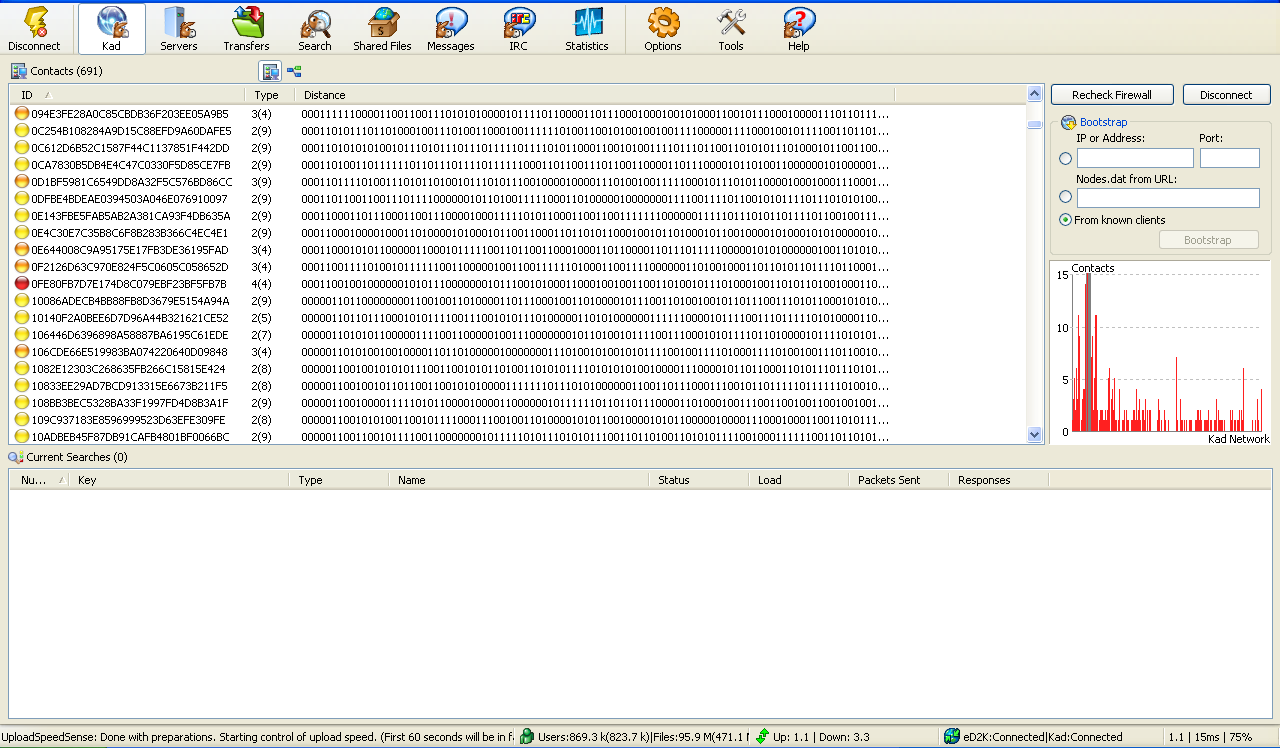
\includegraphics[width=0.8\textwidth]{kadwindow.png}
		\caption{\label{kadwindow}A janela de conexão via Kad Network.}
	\end{figure}
    
    


	\subsection{Funcionamento da conexão entre dois nós}
		A busca por uma determinada informação ou usuário (não importa o que se busque) sempre passará pela mesma função hash de 
definição de nós, que retornará um identificador; a partir daí, o nó que gerou a requisição deve fazer um XOR de seu identificador com 
esse novo, produzindo um valor que determinará qual será o próximo nó que a mensagem será roteada. Tabelas de roteamento também são 
implementadas com o Kademlia, consistindo de uma lista (ou \textit{k-bucket}) contendo k-nós; do resultado do XOR, esses baldes são 
verificados para definir se o nó atual conhece esse identificador ou se ele deve roteá-lo para um nó conhecido que esteja mais próximo.

		A  utilização de DHT, no caso da rede eD2k, se aplica entre os supernós, funcionando basicamente da mesma maneira; porém, 
o nó que faz a requisição irá escolher entre busca local (ou seja, somente entre os nós que o supernó conhece) ou busca global. Nesse 
último caso, o supernó (ou servidor) irá realizar a busca através de DHT com outros supernós conhecidos. Quando o nó destino recebe a 
mensagem, o estabelecimento de conexão é feito através de um protocolo TCP, e a fila de downloads é verifica: quando ela for vazia, a 
troca de informações entre esses dois nós terá início. A quantidade mínima da taxa de download de ambos deve ser maior que 2kbytes/sec, 
portanto caso seja possível, um cliente pode, enquanto troca dados com esse nó, estar conectado e fazendo transferência de arquivos com 
outros nós, desde que essa taxa seja respeitada. A quantidade de fontes para download é mostrada para o usuário, na janela de 
transferência de arquivos.

	\subsection{Recuperação de diferentes partições de um arquivo}
    	Como dito anteriormente, cada arquivo introduzido na rede passa por uma função de hash, onde é definido seu ID, e para facilitar a transferência das partes ele é dividido em partes menores de aproximadamente 9.25 MB. 
        Uma vez que a conexão entre os dois nós é realizada, o download começa e as partes dos arquivos são baixadas separadamente.
        Existem opções no próprio eMule que permitem a checagem que garante que as partes do arquivo que foram baixadas vieram completas, e no caso de corrompimento, é possível refazer o download apenas da parte que veio corrompida. Quando todas as partes são baixadas e conferidas, o eMule faz o trabalho de juntar elas e formar o arquivo final, que é disponibilizado ao usuário. É importante lembrar que a partir do momento que uma parte é totalmente transferida ao cliente, este pode servir de distribuidor dessa parte para outros usuários, mesmo que o arquivo não esteja 100\% completo.
        
        Na tela de transferência de arquivos do eMule, é possível verificar quais arquivos estão sendo baixados ou compartilhados e quantas fontes estão envolvidas nessas duas transações. É possível também assegurar-se de qual tipo de conexão está sendo estabelecida - via eD2k ou Kad Network.

	\subsection{Saída da rede}\
	Quando o eMule é fechado, o usuário é desconectado da rede, interrompendo assim qualquer transferencia de arquivo que está sendo realizada (seja upload ou download). No caso do ed2k, o servidor reconhece que o usuário foi desconectado e para de indicá-lo como fonte de arquivos. Usando o Kademlia a rede é automaticamente organizada, já que de tempos em tempos os nós realizam a verificação para saber se os nós vizinhos ainda existem e se nós novos foram acrescentados (como citamos na sessão Entrada na Rede).
    
 	\subsection{Ofuscação na rede}\
	Um dos recursos interessantes que estão disponíveis no eMule a partir da versão 0.47b é o Protrocolo de  Ofuscação. Com ele é possível fazer com que os pacotes enviados pelo eMule não sejam identificados como tais automaticamente quando são transmitidos pela rede. Essa característica serve para facilitar a troca de dados quando o protocolo do eMule é parcialmente discriminado ou totalmente bloqueado em determinada rede; entretanto é importante lembrar que essa função não deixa o usuário invisível na rede. 
    
    Sempre é possível rastrear o pacote, mas com a ofuscação os dados vem de maneira aleatória no pacote, sendo difícil de identificá-lo sem uma verificação mais completa. A Ofuscação está disponível para as conexões TCP e UDP da rede eD2k, TCP e UDP com os servidores e conexões TCP da Kad. Pacotes UDP da rede Kademlia ainda não estão sendo ofuscados. 
    \subsection
    {Sistema de créditos}\
    Uma outra caracteristica presente no eMule é o sistema de créditos, que funciona como uma recompensa para usuários ativos do sistema e que contribuem principalmente com o upload de arquivos. O crédito funciona como um modificador no cálculo da posição da fila de cada usuário. Existem duas razões modificadoras: 
    Razão 1 = Upload Total x 2 / Download Total
  	Razão 2 = SQRT(Upload Total + 2)
    
Ambas as razões são comparadas e o valor mais baixo é utilizado como modificador. Portanto, quanto maior a quantidade de upload, mais benefício na fila o usuário terá. É importante ressaltar que os créditos de um usuário são guardados junto ao nó que está recebendo a transferência de upload, para que se previna a falsificação de crédidos. Não é possível saber qual a quantidade de créditos que você possui. Vale lembrar também que os créditos não são globais, e sim uma relação entre cada par de nós.

\section{Considerações finais}
	Apesar de ser um sistema de mais de dez anos, o eMule ainda persiste como um dos mais utilizados P2P da atualidade, competindo com grandes nomes da atualidade como o BitTorrent. Seu sistema de busca de arquivos ainda é bastante tradicional em comparação ao seu concorrente previamente citado - no caso de uma conexão eD2k, servidores são consultados, e na Kad Network a DHT é consolidada para a busca de um arquivo. Mesmo sendo algo que, em teoria, é funcional, esse processo algumas vezes se torna difícil, visto que a quantidade de usuários ingressos em redes suportadas pelo eMule vem diminuindo ao longo dos anos.
    
    Outras características fazem o eMule ser prejudicado em sua avaliação geral. Em uma era onde acontece uma clara transição entre o protocolo IPv4 para o IPv6, o programa não oferece suporte a esse último, o que pode ser um problema no futuro. A quantidade de atualizações também é escassa - a última foi em 2010, cerca de 5 anos atrás, ao passo que atualizações ocorrem com grande frequência em aplicações que utilizam o BitTorrent como protocolo. Uma outra desvantagem dessa própria infra-estrutura de comunicação é a ausência de um sistema de reputação, o que poderia aliviar a transferência de arquivos maliciosos ou mal-intencionados - alguns servidores eD2k são considerados falsos (\textit{fake}), estando ali somente para fins mal-intencionados ou para análise de tráfego de arquivos.
    
    Apesar de todas essas informações, o eMule ainda é bastante popular, e sua utilização é muito abrangente.


    
    
\section{Fontes}
	\url{http://www.emule-project.net}
    \url{http://www.afterdawn.com/guides/archive/little_emule_tutorial.cfm#0337}
	
\end{document}
